\documentclass[11pt,final,oneside]{fithesis}
\usepackage[utf8]{inputenc}
\usepackage[T1]{fontenc}
\usepackage{tipa}
\usepackage[slovak]{babel}
\usepackage{tabularx}
\usepackage{graphicx}
\usepackage{cite}
\usepackage{url}

\hbadness=1000
\tolerance=1000

\newcommand{\smalltt}[1]{\small\texttt{#1}\normalsize}

\thesistitle{Monitorování zátěže a využití výpočetních zdrojů v heterogenním výpočetním prostředí}
\thesissubtitle{Diplomová práca}
\thesisstudent{Juraj Leždík}
\thesiswoman{false}
\thesisfaculty{fi}
\thesisyear{jar 2016}
\thesisadvisor{Mgr. Miroslav Ruda}
\thesislang{sk}
\begin{document}

\FrontMatter
\ThesisTitlePage

\begin{ThesisDeclaration}
\DeclarationText
\AdvisorName
\end{ThesisDeclaration}


\begin{ThesisThanks}
\end{ThesisThanks}

\begin{ThesisAbstract}
\end{ThesisAbstract}

\begin{ThesisKeyWords}
\end{ThesisKeyWords}

\tableofcontents
\addcontentsline{toc}{chapter}{Obsah}

\MainMatter
\chapter{Úvod}

\chapter{OpenTSDB}
OpenTSDB pozostáva z Time Series Daemon (TSD) a z utilít pre príkazový riadok. Interakcia s OpenTSDB je primárne realizovaná cez jedného alebo viacerých TSD. Každý TSD je nezávislý.
Neexistuje žiadny riadiaci proces, žiadny zdieľaný stav, takže je možné spustiť toľko TSD, koľko je potrebné na zvládnutie požadovanej záťaže. Každý TSD používa open-source databázu HBase
na ukladanie a vyberanie dát časových rád. HBase schéma je vysoko optimalizovaná na rýchlu agregáciu podobných časových rád, aby minimalizovala požiadavky na úložný priestor. 
Používatelia TSD nemusia kpristupovať do HBase priamo. S TSD je možné komunikovať cez jednoduchý protokol podobný Telnetu, cez HTTP API alebo cez jednoduché GUI. Všetka komunikácia
sa deje na tom istom porte (TSD odhadne protokol klienta pohľadom na prvých niekoľko bajtov, ktoré obdrží).\cite{openTSDB}


\chapter{Oblasti monitorovania}
\section{Torque}
TORQUE Resource Manager poskytuje kontrolu nad dávkovými úlohami a distribuovanými výpočetnými zdrojmi. Je to pokročilý open-source product, založený na na pôvodnom PBS projekte. 
Zahŕňa vyznamné pokroky v oblastiach škálovania, spoľahlivosti a funkcionality a je v súčasnosti používaný desiatkami tisícov vládnych, akademických a komerčných webových stránok po celom svete. Torque môže byť voľne používaný, modifikovaný a distribuovaný je v rámci obmedzení svojou licenciou.\cite{torque}

Monitorovanie tejto aplikácie bude prebiehat prostredníctvom volania jej ovládacích príkazov:
\begin{description}
\item[\emph{momctl}] - sledovanie záťaže riadiaceho procesu a zisťovanie, ktoré úlohy sa práve spracovávajú
\item[\emph{printjob}] - sledovanie zdrojov, ktoré spotrebováva konkrétna úloha 
\end{description}

\section{libvirt/KVM}
KVM\footnotemark\footnotetext{Kernel-based Virtual Machine} je plné virtualizačné riešenie pre Linux pre x86 hardvér, obsahujúce virtualizačné rozšírenia (Intel VT or AMD-V).
Pozostáva z nahrateľného modulu jadra, kvm.ko, ktorý poskytuje základ virtualizačnej infraštruktúry a šepcifický modul, kvm-intel.ko alebo kvm-amd.ko. Je možné virtualizovať obrazy 
s operačným systémami Linux aj Windows. Každý virtuálny stroj má vlastný virtualizovaný hardvér: sieťovú kartu, disk, grafický adaptér, atď. KVM je open-source softvér. Virtualizačný modul jadra
sa nachádza v Linuxe od verzie 2.6.20.\cite{torque}

libvirt je sada nástrojov na prácu s virtualizačnými schopnosťami Linuxu (a ostatných OS). Je to voľný softvér dostupný pod licenciou GNU LGPL. 
Obsahuje API v jazyku C a väzby pre bežné programovacie jazyky.\cite{libvirt}

Na monitorovanie virtuálnych strojov použijem API libvirt v jazyku Python. Budem sledovať využívanie nasledujúcich zdrojov vo virtuálnom stroji:
\begin{description}
\item[\emph{procesor}]
\item[\emph{pevný disk}]
\item[\emph{sieť}]
\end{description}

libvirt momentálne neposkytuje nástroje na monitorovanie spotreby pamäte.


Využijem už existujúcu implementáciu sond na zber týchto údajov (aspoň teda myslím).

\section{Docker}
Docker umožňuje zabaliť aplikáciu so všetkými jej závislosťami do štandardizovanej jednotky určenej na softvérový vývoj. Kontajnery Dockeru obaľujú softvér kompletným súborovým systémom, ktorý
zahŕňa všetko, čo daný softvér potrebuje na spustenie: kód, nástroje potrebné na beh, systémové nástroje a knižnice. Toto zaručuje, že program bude pracovať rovnako bez ohľadu na prostredie, v ktorom
je spustený.\cite{docker}

\subsection{Porovnanie s virtuálnymi strojmi}
Kontajnery predstavujú podobný prístup ako virtualizácia. Tiež ide o snahu spúšťať softvér v prostredí oddelenom od skutočného hardvéru a operačného systému. Na rozdiel od úplných virtuálnych strojov 
nie je virtualizovaný celý hardvér, ale len softvérové vybavenie nevyhnutné na spustenie programu. Rozdiel v architektúre ilustruje nasledovný obrázok: 
\begin{figure}[h]
\begin{center}
       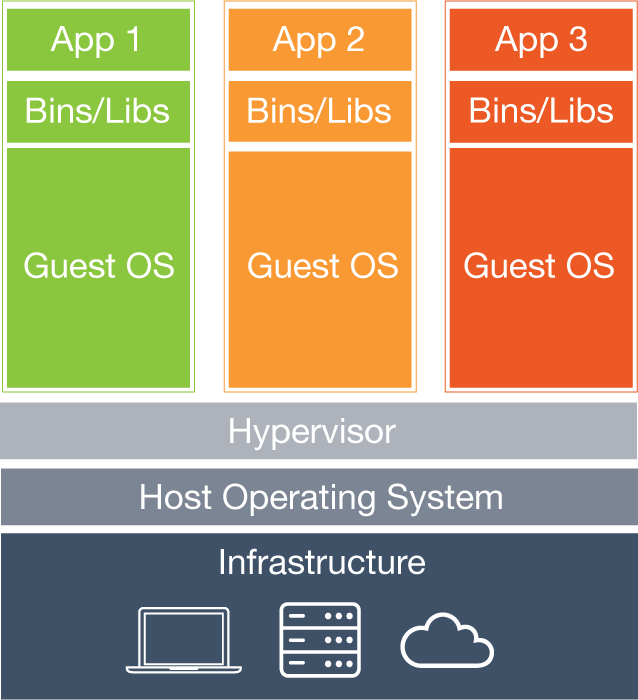
\includegraphics[width=0.8\textwidth]{images/docker.png}
       \caption{Porovnanie architektúry Docker a virtuálnych strojov}\cite{docker}
\end{center}
\end{figure}

\subsection{Komunikácia s Dockerom}
Na komunikáciu s Dockerom je možné využiť:
\begin{description}
\item[príkazy aplikácie v príkazovom riadku]
\item[Remote API]
\end{description}

Používanie príkazov aplikácie môže byť o čosi rýchlejšie, ale následne by bolo potrebné analyzovať textový výstup programu.
Rozhodol som sa použiť Remote API. Toto API funguje pre účely monitorovania na princípe REST a odpovede vracia vo formáte JSON, čo predstavuje zjednodušenie spracovania výstupu. Démon Dockeru "počúva" na 
lokálnom sockete, čo by nemalo spôsobovať výrazné oneskorenie odpovede.

O každom kontajneri spustenom v Dockeri budem sledovať využívanie týchto zdrojov :
\begin{description}
\item[\emph{procesor}]
\item[\emph{pevný disk}]
\item[\emph{sieť}]
\item[\emph{pamäť}]
\end{description}

Príklad odpovede - pre orientáciu, aké dáta sa dajú zberať:
\\  HTTP/1.1 200 OK
\\  Content-Type: application/json
\\
\\  \{
\\     "read" : "2015-01-08T22:57:31.547920715Z",
\\     "networks": \{
\\            "eth0": \{
\\                 "rx_bytes": 5338,
\\                 "rx_dropped": 0,
\\                 "rx_errors": 0,
\\                 "rx_packets": 36,
\\                 "tx_bytes": 648,
\\                 "tx_dropped": 0,
\\                 "tx_errors": 0,
\\                 "tx_packets": 8
\\             \},
\\             "eth5": \{
\\                 "rx_bytes": 4641,
\\                 "rx_dropped": 0,
\\                 "rx_errors": 0,
\\                 "rx_packets": 26,
\\                 "tx_bytes": 690,
\\                 "tx_dropped": 0,
\\                 "tx_errors": 0,
\\                 "tx_packets": 9
\\             \}
\\     \},
\\     "memory_stats" : \{
\\        "stats" : \{
\\           "total_pgmajfault" : 0,
\\           "cache" : 0,
\\           "mapped_file" : 0,
\\           "total_inactive_file" : 0,
\\           "pgpgout" : 414,
\\           "rss" : 6537216,
\\           "total_mapped_file" : 0,
\\           "writeback" : 0,
\\           "unevictable" : 0,
\\           "pgpgin" : 477,
\\           "total_unevictable" : 0,
\\           "pgmajfault" : 0,
\\           "total_rss" : 6537216,
\\           "total_rss_huge" : 6291456,
\\           "total_writeback" : 0,
\\           "total_inactive_anon" : 0,
\\           "rss_huge" : 6291456,
\\           "hierarchical_memory_limit" : 67108864,
\\           "total_pgfault" : 964,
\\           "total_active_file" : 0,
\\           "active_anon" : 6537216,
\\           "total_active_anon" : 6537216,
\\           "total_pgpgout" : 414,
\\           "total_cache" : 0,
\\           "inactive_anon" : 0,
\\           "active_file" : 0,
\\           "pgfault" : 964,
\\           "inactive_file" : 0,
\\           "total_pgpgin" : 477
\\        \},
\\        "max_usage" : 6651904,
\\        "usage" : 6537216,
\\        "failcnt" : 0,
\\        "limit" : 67108864
\\     \},
\\     "blkio_stats" : \{\},
\\     "cpu_stats" : \{
\\        "cpu_usage" : \{
\\           "percpu_usage" : \[
\\              16970827,
\\              1839451,
\\              7107380,
\\              10571290
\\           \],
\\           "usage_in_usermode" : 10000000,
\\           "total_usage" : 36488948,
\\           "usage_in_kernelmode" : 20000000
\\        \},
\\        "system_cpu_usage" : 20091722000000000,
\\        "throttling_data" : \{\}
\\     \}
\\  \}
  
Dáta je možné zberať buď ako prúd, alebo po jednorazových žiadostiach. To ešte nemám veľmi preštudované, neviem aké sú tam intervaly, tak sa rozhodnem až neskôr.
Predpokladám ale, že z hľadiska rýchlosti a alokácie bude cesta asi ten stream.


Sonda pre Docker bude napísaná v Go.
\section{Hadoop}
Projekt Apache™ Hadoop® vyvíja open-source softvér na spoľahlivé, škálovateľné, distribuované výpočty. Apache Hadoop je prostredie, ktoré umožňuje distribuované spracovávanie veľkých množstiev dát
naprieč clustermi, používajúcimi jednoduché programovacie modely. Je navrhnutý tak, aby bol škálovateľný od jednotlivých serverov po tisícky strojov, kde každý poskytuje lokálny výpočetný výkon a úložný priestor.
Nespolieha sa na vysokú dosupnosť hardvérových prostriedkov, ale je navrhnutý, aby detekoval a zvládal chyby na aplikačnej vrstve, takže poskytuje vysoko dostupnú službu nad clusterom počítačov, z ktorých 
každý je náchylný na chyby.

Projekt pozostáva z týchto modulov:

\begin{description}
\item[\emph{Hadoop Common:}] spoločné nástroje, ktoré podporujú ostatné Hadoop moduly
\item[\emph{Hadoop Distributed File System (HDFS™):}] distribuovaný súborový systém, ktorý poskytuje vysokú priepustnosť
\item[\emph{Hadoop YARN:}] prostredie pre plánovanie úloh a správu zdrojov clustera
\item[\emph{Hadoop MapReduce:}] systém založený na YARN pre paralelné spracovávanie veľkých množstiev dátprostredie pre plánovanie úloh a správu zdrojov clustera
\end{description}

K monitorovaniu len toľko, čo viem z materiálov, čo som dostal do mailu. Že existuje REST API, ktoré je ale trochu pomalé, a že štatistiky sa ukaladajú aj niekam na HDFS, ale zrejme v nejakom XML interného
formátu. Takisto by som potreboval skonzultovať, že čo vlastne monitorovať.

\chapter{Návrh}
Monitorovacia aplikácia bude pozostávať z dvoch častí. Jednou bude manažér a druhou monitorovacie sondy. Manažér bude oslovovať jednotlivé sondy v pravidelných intervaloch, aby mu poslali údaje o zaťažení.
Tieto údaje následne bude odosielať TSD. Manažér bude napísaný v Go a bude využívať Go rutiny (niečo ako vlákna) - jednu pre každú sondu.

V prípade napr. toho Torque sme sa bavili, že je možné, že na dotaz o zaťažení môže trvať v niektorých prípadoch aj polhodinu, kým príde odpoveď. V princípe nejde nijako odlíšiť, či daná sonda čaká na údaje
alebo sa zasekla. Preto každá sonda bude obsahovať časť, ktorá bude stále živá a bude komunikovať s manažérom. Buď mu pošle nové údaje, alebo povie, že čaká. V tom prípade manažér použije poslednú hodnotu.
V prípade, že sonda bude čakať na údaj, nebudú sa vytvárať nové požiadavky na tento údaj. Opätovný dotaz na údaje bude vytvorený až po uplynutí nejakého časového intervalu a starý dotaz bude zrušený/ukončený.
Tento časový interval si bude môcť užívateľ nastaviť pre každú sondu. Zároveň by som chcel ale otestovať v reálnom prostredí, aký interval by bol vhodný pre tú ktorú sondu.

Ďalšou vecou na riešenie by bolo zabezpečenie dát. To ale momentálne nie je podporované v OpenTSDB, tak by šlo len o teoretické rozobratie. Ďalšie nové veci, už teraz nevymyslím, najprv treba niečo nakódiť
a objaviť komplikácie.

\chapter{Záver}

\bibliographystyle{csplainurl}
\nocite{*}
\bibliography{dip-lezdik}
\addcontentsline{toc}{chapter}{Literatúra}

\begin{appendix}
\chapter{Kapitola priloha}
\end{appendix}

\end{document}
